% coding:utf-8

%----------------------------------------
%FOSAPHY, a LaTeX-Code for a summary of basic physics
%Copyright (C) 2013, Mario Felder, Michael Fallegger

%This program is free software; you can redistribute it and/or
%modify it under the terms of the GNU General Public License
%as published by the Free Software Foundation; either version 2
%of the License, or (at your option) any later version.

%This program is distributed in the hope that it will be useful,
%but WITHOUT ANY WARRANTY; without even the implied warranty of
%MERCHANTABILITY or FITNESS FOR A PARTICULAR PURPOSE.  See the
%GNU General Public License for more details.
%----------------------------------------

\chapter{Wärme}

\section{Konstanten}
\[
\boxed{\begin{aligned}	
		&\text{Avogadrozahl} \\
		&N_{A} = 6.00221 \cdot 10^{23}\text{ Teilchen}\\
		\\
		&\text{Universelle Gaskonstante}\\
		&R = 8.314472 \frac{J}{mol \cdot K}\\
		\\
		&\text{Boltzmann}\\
		&k_{B} = \frac{R}{N_{A}}=1.381 \cdot 10^{-23} \frac{J}{K}
	\end{aligned}}	\]

\section{Ideale Gasgleichung}

\[pV = nRT = \frac{N_{tot}}{N_{A}}RT = \frac{m_{tot}}{m_{mol}}RT\]

\begin{tabular*}{\linewidth}{p{0.15\linewidth}lp{0.37\linewidth}}
	\textbf{Variable}				&	\textbf{Bedeutung}		& \textbf{Einheit}\\
	\hline
	\rowcolor{white}$p$			&      Gasdruck				&$Pa$\\
	\rowcolor{lgray}$T$			&	Gastemperatur			& $K$\\
	\rowcolor{white}$N_{tot}$	&	Anzahl Moleküle im Gas	&$ $\\				
	\rowcolor{lgray}$m_{tot}$	&	Gasmasse				&$ $\\
	\rowcolor{white}$n$			&	Anzahl mol im Gas		&$ $\\
	\rowcolor{lgray}$N_{A}$		&	Avogadrozahl			&$N_{A} = 6.022 \cdot 10^{23} \frac{Teilchen}{mol}$\\	
	\rowcolor{white}$m_{mol}$	&	Molmasse				&$ $\\
\end{tabular*}


\section{Luftdruck vs. Höhe bei konstanter Temperatur}
Der Schweredruck in einm Fluid ist $\Delta p=-\rho \cdot g\Delta y$.\\

\[
\boxed{\begin{aligned}	
		p(y)&=p_0 \cdot \e^{- \frac{m_{mol}g}{RT}y} = p_0 \e^{-\frac{y}{H}}
		\\
		H&= \frac{RT}{m_{mol}g}
	\end{aligned}}\]
\begin{footnotesize}
	$H$: charakteristische Höhe (analog zu Zerfallszeit $\tau$)
\end{footnotesize}


\section{Luftdruck bei veränderlicher Temperatur}
Troposphäre ($0-11km$):
\[\begin{aligned}
	T &= a - b \cdot y \\
	a &= 15^\circ C\\
	b &= 6.5 \frac{^\circ C}{km}
\end{aligned}\]
\\
Druck:
\[
	p = p_0 \left( \frac{a-b \cdot y}{a} \right)^{\frac{m_molg}{R\cdot b}} = p_0 \left( \frac{T}{T_0} \right)^{\frac{m_molg}{R\cdot b}}
\]


\section{Energie}

Kinetische Energie im idealen Gas.
	\[ E_{Gas} =\frac{3}{2}nRT\]
\newline
Mittlere kinetische Energie eines Moleküls im idealen Gas.
	\[ \langle E_{kin, k\"ul} \rangle = \frac{1}{2}m_{k\"ul} \langle v^2 \rangle = \frac{3}{2}k_{B}T\]
\newline



\section{Geschwindigkeiten}
\[
	v_{rms}= \sqrt{\langle v^2\rangle}
	=\sqrt{\frac{3k_BT}{m_{kül}}}=\sqrt{\frac{3RT}{m_{mol}}}
\]
\\
Wahrscheinlichste Geschwindigkeit:
\[
	v_{w}=\sqrt{\frac{2k_{B}T}{m_{k\"ul}}}=\sqrt{\frac{2RT}{m_{mol}}}
\]
\\
Durchschnittsgeschwindigkeit:
\[
	v_{av}=\sqrt{\frac{8k_{B}T}{\pi m_{k\"ul}}}=\sqrt{\frac{8RT}{\pi m_{mol}}}
\]
\newline


\section{Freiheitsgrade FG}
Das einatomige, ideale Gas hat genau drei Bewegungs-Freiheitgrade: links nach rechts, hinten nach vorn, unten nach oben. Zweiatomige Gase haben mehr Bewegungsmöglichkeiten.\\
\\
\textbf{Äquipartitions Gesetz} der klassischen Mechanik:\\ 
Auf jeden aktiven Freiheitsgrad eines Moleküls in einem Gas der Temperatur $T$ entfällt im Mittel die Energie $\frac{1}{2}k_{B}T$.

\[\boxed{\begin{aligned}
		\frac{\langle E_{kül} \rangle}{FG}&= \frac{1}{2}k_{B}T
		\\
		\frac{\langle E_{mol} \rangle}{FG}&= \frac{1}{2}R \cdot T
	\end{aligned}}\]	

\section{Spezifische Wärmekapazität c}
Um die Temperatur einer Substanz zu erhöhen, kann man ihr Wärme Q zuführen. Wärme ist eine Energieform [J]. Eine Kalorie entspricht $4.186J$.


\[\boxed{
	\begin{aligned}
		Q&=m \cdot c \cdot \Delta T \rightarrow \di Q=m \cdot c \cdot \di T
		\\
		\text{c pro Masse: }c_{(m)}&=\frac{1}{m} \difrac{Q}{T}
		\\
		\text{c pro Mol: }c_{(n)}&=\frac{1}{n} \difrac{Q}{T}		
		\\
		c_{(m)}&=\frac{c_{(n)}}{m_{mol}}
	\end{aligned}	
	}\]	
\\	
Spezifische Wärmekapazität des \textbf{idealen Gases} pro Mol, bei $\underline{\mathrm{konstantem}}$ Gasvolumen.
\\
\\		Einatomigen Gases:
		\[\boxed{			
			c_{(n)V}=C_{V}=\frac{3}{2}R
		}\]\newline
		Zweiatomigen Gases:
		\[\boxed{	
			c_{(n)V}=C_{V}=\frac{5}{2}R							
		}\]\newline

\section{Mittlere freie Weglänge $\Lambda$}
Wir betrachten die Moleküle alas harte Kugeln mit Radius $r$ und leiten eine Kollisionszeit $t_{mean}$ und eine mittlere freie Weglänge $\Lambda$ her.\\
\\
Mittlere Kollisionszeit
\[ t_{mean} = \frac{dt}{dN}= \frac{V}{4 \pi \sqrt{2} \cdot r^2vN} \]
\\	
Mittlere freie Wegl\"ange
\[ \Lambda =v \cdot t_{mean}= \frac{V}{4 \pi \sqrt{2} \cdot r^2 \cdot N}=  \frac{k_{B} \cdot T}{4 \pi \sqrt{2} \cdot r^2 \cdot p} \]

\section{Wahrscheinlichkeit}
Die Verteilfunktion der molekularen Geschwindigkeiten f(v) kann mittels statistischer Mechanik hergeleitet werden.\\
\\
Maxwell-Boltzmann Verteilung
\[ f(v)=4\pi \left(\frac{m_{mol}}{2\pi \cdot RT}\right)^{\frac32} \cdot v^2 \cdot \e^{-\frac{m_{mol} \cdot v^2}{2RT}}\]

\[ f(v)= 4\pi \left(\frac{m_{kül}}{2\pi \cdot k_{B}T}\right)^{\frac32} \cdot v^2 \cdot \e^{-\frac{m_{kul} \cdot v^2}{2k_{B}T}}\]
\\
Wahrscheinlichkeitsdichte:
\[ W(v_{1},v_{2})= \int\limits_{v_{1}}^{v_{2}} f(v)\di v\]

\[ W(v_{1},v_{2})= \int\limits_{v_{1}}^{v_{2}} 4\pi \left(\frac{m_{mol}}{2\pi \cdot RT}\right)^{\frac32} \cdot v^2 \cdot \e^{-\frac{m_{mol} \cdot v^2}{2RT}}\di v\]
\\
Energie-Verteilfunktion:
\[
	W(E_1, E_2) = \int\limits_{E_1}^{E_2} \frac{8\pi}{\sqrt{2}} \left( \frac{1}{2\pi k_B T} \right)^\frac32 \sqrt{2} \cdot \e^{-\frac{E}{k_B T}} \di E
\]

\section{Volumenarbeit eines Gases}
Das Vorzeichen stellt sicher, dass das Gas bei Expansion $(V_2>V_1)$ Arbeit an der Aussenwelt verrichtet. Die Arbeit W ist bei Expansion negativ und geht aus dem Gas heraus, das Gas verliert Energie!

\[\boxed{
	W=-\int_{V_1}^{V_2}p\cdot dV
}\]

\section{Innere Energie U, Erster Hauptsatz der TD}
Die innere Energie U eines Körpers ist eine Zustandsgrösse der Thermodynamik. Sie setzt sich zusammen aus der kinetischen ("Zittern") und der potentiellen Energie ("Federn") aller Moleküle des Körpers vorstellen. Der erste Hauptsatz der Thermodynamik besagt: Die innere Energie vergrössert sich mit Zufuhr von Wärme und/oder Arbeit.

\[\boxed{
	\Delta U_{U_2-U_1}= Q_{in}+W_{in} \qquad \di U=\di Q_{in}+\di W_{in}=\di Q-p \cdot \di V	
}\]
\\
\subsection{Innere Energie des idealen Gases}
Innere Energie des idealen Gas:\\
\[\boxed{
	U=U(T)=n\underbrace{\frac{FG}{2}R}_{C_V} T=nC_VT
}\]
\\
\begin{tabbing}
	Freiheitsgrade:\qquad= 3 für einatomiges Gas\\
	Freiheitsgrade:\qquad\=\kill
	\> = 5 für zweiatomiges Gas
\end{tabbing}

\newpage

\subsection{Zustandsänderungen des idealen Gas}
\begin{figure}[h!]
	\begin{center}
		\leavevmode
		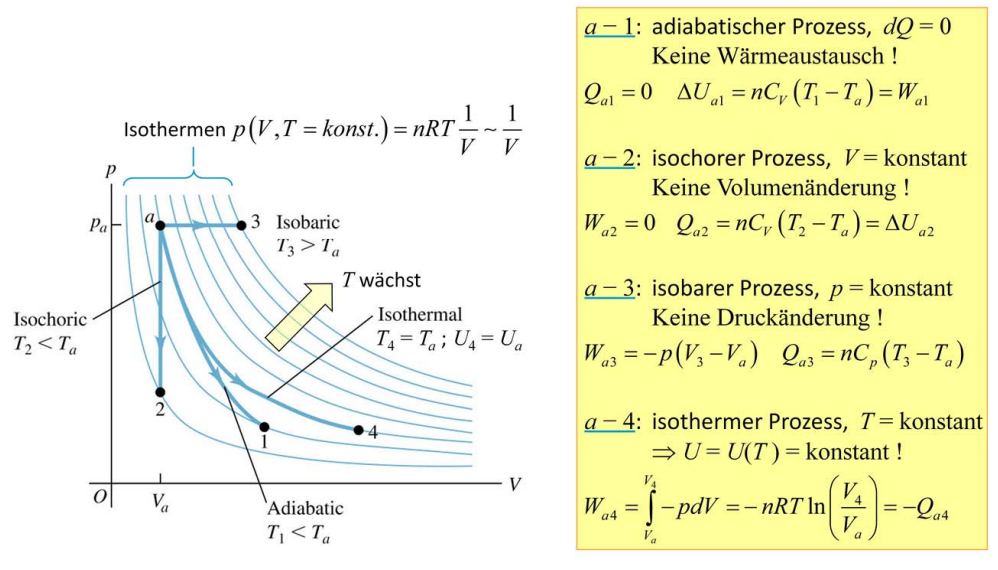
\includegraphics[scale=0.42, trim = 0mm 0mm 0mm 0mm, clip]{../fig/zustandsaenderung.png}
		\caption{Zustandsänderung}
	\end{center}
\end{figure}
adiabatisch = isotrop
\\

\subsection{Spezifische Wärme $C_p$ des idealen Gas}
Molare Wärmekapazitäten des idealen Gas:
\[\boxed{
	C_p=C_V+R
}\]
Verhältnis der molaren Wärmekapazitäten des idealen Gas:
\[\boxed{
	\gamma = \frac{C_p}{C_V}=\frac{C_V+R}{C_V}=
	\begin{aligned}
		\left\{
		\begin{array}{l l}
			& 1.67 \quad  1-atomiges Gas  \\ 
			& 1.40 \quad  2-atomiges Gas
		\end{array}
		\right\}
	\end{aligned}
}\]

\subsection{Adiabatischer Prozess des idealen Gas}
Das System ist thermisch isoliert. Eine Temperaturänderung stammt immer von einer Arbeit, nicht von einem Wärmefluss $\rightarrow$ $\Delta U=W$ ($Q=0$)
\\
\[\boxed{
	\begin{aligned}
	T_1\cdot V_1^{\gamma-1} &= T_2\cdot V_2^{\gamma-1}\\ 
	p_1\cdot V_1^{\gamma} &= p_2\cdot V_2^{\gamma} \\
	T_1\cdotp p_1^{\frac{1-\gamma}{\gamma}} &= T_2\cdot p_2^{\frac{1-\gamma}{\gamma}}\\
	\\\\
	\Delta U=nC_V(T_2-T_1)&=W=\frac{p_2V_2-p_1V_1}{\gamma-1}
	\end{aligned}	
}\]

